
\section{Motivation}
\label{sec:motivation}

The research project focuses on identifying the mismatch and
opportunities for improvement between commodity operating systems and
a large, but well-defined, class of relevant applications.  In this
section, we first define the class of applications in our focus
(\S\ref{sec:motivation:web}), then describe the system software
challenges associated with that class of applications
(\S\ref{sec:motivation:challenges}), and identify an alternative model --
the dataplane -- which addresses these challenges
(\S\ref{sec:motivation:dp}.

\subsection{Event-driven, web-scale applications}
\label{sec:motivation:web}

Today's web-scale applications, which our lives have grown accustomed
to to retrieve information (search), communicate (email, instant
message), share (social networking) or buy (e-tailers) simultaneously
offer quick response times to millions of concurrent users, while
accessing massive data sets spread out over thousands of servers.
Today's interactive web-scale applications have further redefined
expectations of responsiveness. For example, the Google search engine
updates query results interactively as the user types, predicting the
most likely query based on the prefix typed so far, performing the
search and showing the results within a few tens of
milliseconds~\cite{DBLP:journals/cacm/DeanB13}.

Internally, such applications are deployed on thousands of servers
operating distinct, well-defined services, such as load-balancing,
application serving, content distribution and streaming, memory
caching, relational databases and object storage~\cite{missing}.  In
addition, web-scale applications also rely on massive, batch-oriented
services that prepare the data for interactive serving (e.g., the
search engine crawlers), identify patterns and behavior from the
massive data sets and the users' behaviors via machine
learning~\cite{missing}.  Because of this diversity, different
services are routinely implemented using different programming
languages, framework and paradigms.

The event-driven paradigm is the most commonly used for services that
are directly involved in serving interactive applications.  In this
paradigm, each application node is primarily responding to external
events such as a new incoming connections, a request from an incoming
connection, or a reply to a request made to a downstream service.
This category includes stateless load balancers, HTTP proxies, web
servers, application severs, key-value stores, queuing services,
caching servers, and many others.  

For each category, the most efficient implementations today are
implemented using event-driven frameworks in which application logic
interacts with the framework exclusively via non-blocking calls.  This
is in contrast with the classic thread-oriented programming paradigm,
in which sessions are divided among a large pool of (kernel)
threads, which block while waiting for incoming traffic or outstanding
replies.  For example, the event-oriented nginx HTTP
server and proxy~\cite{reese2008nginx} outperforms the thread-oriented Apache server~\cite{misc:apache}.

Libraries simplify the development of event-driven applications.  For
example, the popular \texttt{libevent} library~\cite{provos2003libevent} provides a level of
abstraction that exposes the paradigm to applications running on top
of Linux, *BSD, and Windows~\cite{missing}.  Many web-scale
applications, including memcached~\cite{missing}, XXX~\cite{missing} are built on top
of libevent.  Others such as Nginx are built using a similar approach.


\subsection{Main Challenges}
\label{sec:motivation:challenges}

Web-scale applications pose unique challenges to system software.
Although the use of an event-oriented paradigm has system-level
benefits, in particular with respect to context switching rates, many
challenges remain that are intrinsic to system software:

\paragraph{Multicore scalability.}

Using today's technology, commodity Xeon processors support 8-10
cores, each consisting of two hyperthreads.  Even when the application
logic is designed to scale and is embarrassingly parallel, the
operating system's networking stack does often become a scalability
bottleneck.

Operating system CPU schedulers were originally designed to
maximize the utilization of the CPU resource among competing
resources.  With the evolution of computer architecture, current
schedulers additionally take cache and memory affinity into
consideration.  Affinity-Accept~\cite{DBLP:conf/eurosys/PesterevSZM12}
improves the affinity of incoming and outgoing network processing by
considering the affinity of flows to core and controlling the NIC
hardware.

Such approaches minimize communication between core but do not
eliminate them.  The lack of
commutativity~\cite{DBLP:conf/sosp/ClementsKZMK13} in the POSIX socket
API implies that cross-core communication is necessary whenever a
connection is accepted or closed.  This poses a significant bottleneck
for workloads that consists of high rates of small, ad-hoc, TCP
connections between servers.  Even with recent kernel improvements that
allow multiple threads to listen to the same socket, (Linux
\texttt{SO\_REUSE)} or ensure flow
affinity~\cite{DBLP:conf/eurosys/PesterevSZM12}, micro-benchmarks
consisting of short TCP-based connections expose first-order
bottlenecks in the operating system.  mTCP~\cite{jeong2014mtcp} does
scale to the maximum number of cores in a socket by running the entire
network stack in userspace in a lock-free manner.


\paragraph{Connection Scalability.}

Connection scalability is the desirable property to support an
increasing number of concurrent connections with no significant impact
on application throughput or latency, up to the memory resource
limitations of the machine.  This has been a historical challenge for
commodity operating systems.  A decade ago, connection scalability
challenges started with as less than 10,000 concurrent
connections~\cite{theC10Kproblem}, which ended up requiring changes to
the kernel and to applications.

Connection scalability remains a challenge today.  For example, the
nature of all-to-all communication between Facebook's application and
memcache servers made it impractical to use TCP sockets between these
two tiers~\cite{nishtala2013scaling}; resulting deployments use a
UDP-based protocol for \texttt{get} operations, and an aggregation
proxy for \texttt{put} operations.

Connection scalability is also a challenge for Internet-facing servers
such as notification services~\cite{DBLP:conf/sosp/AdyaCMP11} and
instant-messaging services.  Indeed, such servers should ideally
support much larger connection counts that for intra-datacenter
communication, as connection capacity becomes the primary metric, and
low-latency and even throughput become secondary.  For example,
WhatsApp Inc. (now part of Facebook) supports up to 2 million concurrent connections on FreeBSD, as
of 2012~\cite{whatsapp-2mil}.  

\paragraph{Micro-second computing}

The notion behind \emph{micro-second computing}~\cite{luiz-isscc} is
that it is essential to minimize the latency of interactions within a
datacenter, and in particular of the remote procedure calls issued by
interactive applications that must access and aggregate massive
amounts of data.  Using today's networking technologies, the typical
communication delay between two servers in a datacenter involves a
pair of 10GE NICs (with a one-way latency as low as
3~\microsecond~\cite{cisco-sereno}), one, three or five cut-through
switches organized in a fat-tree topology (a few hundred $ns$ each, in
the absence of contention, and rapidly shrinking) and propagation
delays (500 $ns$ for 100 meters, with little recent improvements).
Put together, technology enables intrinsic one-way communication
latency of a handful of \microsecond.  

And yet, software ---and in particular system software--- is designed
to operate at a totally different timescale: interrupt coalescing
improve throughput but can delay packets by milliseconds; Queues build
up during device driver processing intervals, introducing noticeable
queuing delays; protocol processing of incoming packets terminates in
the socket layer without directly (or synchronously notifying
applications).  As a result, the remote procedure call latency
observed by application software is one to two orders of magnitude
greater than the intrinsic latency.

\begin{figure}
\begin{centering}
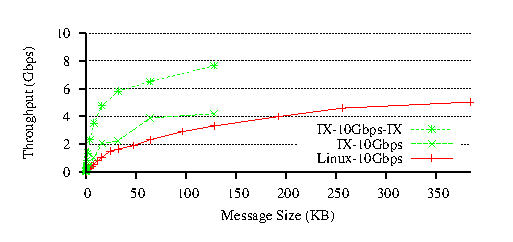
\includegraphics{figs/pingpong.eps}
\caption{NetPIPE performance for varying message sizes and system software configurations.}
\label{fig:pingpong}
\end{centering}
\end{figure}



Fig.~\ref{fig:pingpong} illustrates the importance of system software
design and configuration tradeoffs using a simple ping-pong benchmark
similar to netpipe~\cite{snell1996netpipe} that exchanges a fixed-size
message between two servers.  Although the application is trivial, it
provides a good proxy for the effective performance of synchronous
remote procedure calls in uncontended situations.  We compare the
performance of an out-of-the-box Ubuntu XXX configuration
(\texttt{Linux-base}), a tuned configuration of the same kernel
(\texttt{Linux-opt})), and of our own system (\ix).  For the same
application and hardware configuration (described in
\S\ref{sec:eval:setup}), the differences are dramatic.  This
benchmark is both latency- and bandwdith- sensitive.  We see that \ix
achieves 50\% of the asymptotic bandwdith with messages as small as
\george{XXX bytes}.  In constrast, both Linux configurations remain
latency-bound.


These issues compound when considering the long tail of the latency
distributions~\cite{DBLP:journals/cacm/DeanB13}. Although
tail-tolerance itself is actually an end-to-end problem, the
protocol-processing stacks play a significant role in exacerbating the
problem.  In particular, protocol processing techniques that reduce
latency to microseconds in the common case, but don't improve the 95\%
or 99\% latency are unlikely to result into end-to-end application
gains.

\subsection{The Dataplane Alternative}
\label{sec:motivation:dp}

The main challenges describe above ---multi-core scalability,
connection scalability, and microsecond computing--- are not limited
to event-driven applications operating at large scale.  In fact, such
challenges have been addressed and are reasonably well understood in
others domains.  In particular, middleboxes such as
firewalls~\cite{missing}, load-balancers~\cite{missing}, and software
routers~\cite{DBLP:journals/tocs/KohlerMCJK00,DBLP:conf/sosp/DobrescuEACFIKMR09};
have addresses the problem long ago by integrating the networking
stack and the application into a single \emph{dataplane}.

The solution involves potential tradeoffs in both hardware and
software.  On the hardware side, middlebox services can be deployed
either on commodity Xeon-class servers or virtual machines, or on
processors specifically designed for the networking market.  For
example, Cavium's OCTEON III family of processors offers multiple
100Gbps of external connectivity and 48 64-bit MIPS cores into a
single System-on-Chip~\cite{cavium-octeon}.  This provides increases
energy-efficiencies and densities, at the expense of generality and
volume of the solution.  

On the software side, the typical architecture of a middlebox solution
is designed around the following principles: 

\paragraph{Run to completion.}  Packets are processed ``to
completion'' by the dataplane, eliminating most or all forms of
context switching, system calls, and internal queuing.  In contrast,
the classic kernel construction model generally executes the device
driver code as the result of an interrupt, requires a separate system
call for each segment of a flow received or sent.  The MegaPipe
project~\cite{han2012megapipe} eliminates this latter bottleneck, with
significant benefits.  Furthermore, the POSIX model divides the roles
of the protocol processing stack (which pulls packets from the driver,
de-multiplex them into socket queues, and implements the L3/L4
protocols) and the applications, which asynchronously pull the socket
payload from these queues.  Processing is similar on the transmission
side; in fact, both directions typically require a memory copy.

\paragraph{Coherence-free execution.} 
Different cores operate totally independently
of each other.  In particular common case operations should execute in
a coherence-free manner, i.e., without any cache misses due to the
cache-coherency protocol or any atomic operations that require a
similar access to the cache-coherency layered. This is a much stronger
form of decoupling that the use of locks or of wait-free
synchronization techniques, which have an inherent cache-coherency
traffic cost; 

\paragraph{Embeded deployment model.} 

The software stack is designed to run a single
application, which is directly embedded within the dataplane.  Like
most embedded systems, the application controls all resources, and the
software stack is deployed and operated as a single blob with no
externally-visible distinction between the components.








